\section{Reševanje nerešljivih starogrških problemov}
\label{pogl:starogrskiproblemi}

Z evklidskimi konstrukcijami se je seveda pojavilo konstruktibilnih ugank -- vprašanj, ali sta specifična razdalja ali kot konstruktibilna (in na kakšnen način) ali ne. Stremeli so k iskanju konstrukcij z evklidskim orodjem in če so kakšen problem uspeli rešiti le z neoznačenim ravnilom in šestilom, so te konstrukcije obravnavali kot ``boljše rešitve''~\cite[str. 36]{royster2002}. Grki pa seveda niso delali le s tem orodjem, ampak so se na primer poslužili tudi označenega ravnila\footnote{Martin v trditvi $10.4$ in preko poglavja $9$ v~\cite{geometricconstructions} dokaže, da so origami števila natanko tista množica števil, ki se jih da konstruirati z ravnilom, ki ima na robu dve oznaki.}, s katerim so lahko rešili probleme, ki jih sicer niso mogli. Zelo znani so trije t.\ i.\ ``starogrški' problemi, ki so matematike bremenili več kot tisočletje, začenši s časom Evklida (300 pr.\ Kr.), končno pa sta nanje dokončno odgovorila Niels Henrik Abel (1802--1829) in Evariste Galois (1811--1832) v začetku 19.\ stoletja. Gre za sledeče tri probleme:
\begin{itemize}
    \item \textbf{Podvojitev kocke} Imejmo že konstruktibilno kocko. Konstruiraj novo kocko, ki ima dvakrat večji volumen od prve (problem se poenostavi na iskanje konstrukcije števila $\sqrt[3]{2}$).
    \item \textbf{Trisekcija kota} Dan je poljuben konstruktibilen kot. Konstruiraj kot, ki prvega deli na tri skladne dele.
    \item \textbf{Kvadratura kroga} Za dan konstruktibilen krog konstruiraj kvadrat, ki ima enako ploščino kot dani krog (problem se poenostavi na konstrukcije števila $\sqrt{\pi}$).
\end{itemize}

Z znanjem, ki sta ga znanosti posredovala Abel in Galois, se da pokazati, da ti trije problemi z evklidskim orodjem niso rešljivi. V knjigi o starogrški matematiki od Talesa do Evklida~\cite[str.\ 218--270]{heath1921} je zbrano veliko zamisli in konstrukcij grških matematikov, ki so se ukvarjali s temi tremi problemi in evklidsko orodje ne zadostuje za nobeno od najdenih rešitev.

V nalogi smo do sedaj že večkrat omenili, da pa obstajajo origami konstrukcije (celo več metod za isti problem!), ki nam konstruirajo kubični koren origami števila ter razdelijo kot na tri skladne dele. Vse metode, ki bodo sedaj naštete, zahtevajo uporabo Belochinega pregiba (operacije~\ref{op:O7}), kar je logično, saj so vse ostale origami operacije dovolj za vse evklidske konstrukcije. Žal pa tudi tu ostajamo nemočni glede konstrukcije števila $\sqrt{\pi}$, saj je transcedentno.

\subsection*{Konstrukcija števila $\sqrt{r}$}

Preden si pogledamo konstrukcijo kubičnega korena, vzemimo origami število $r \in $ in kosntruirajmo njegov kvadratni koren (postopek je vzet iz~\cite[str.\ 58]{hull2013}).

Imejmo točko $A (0, 1) $ in premico $y = -1$. Na ordinatni osi označimo točko $B (0, -r/4)$ in z operacijo~\ref{op:O6} skoznjo naredimo pregib, ki točko $A$ položi na premico $y = -1$. Njena zrcalna slika je $A' (t, 0) $ za nek $t \in \R$ (slika~\ref{fig:konstrukcija_korena}).

\begin{figure}[h]
    \centering
    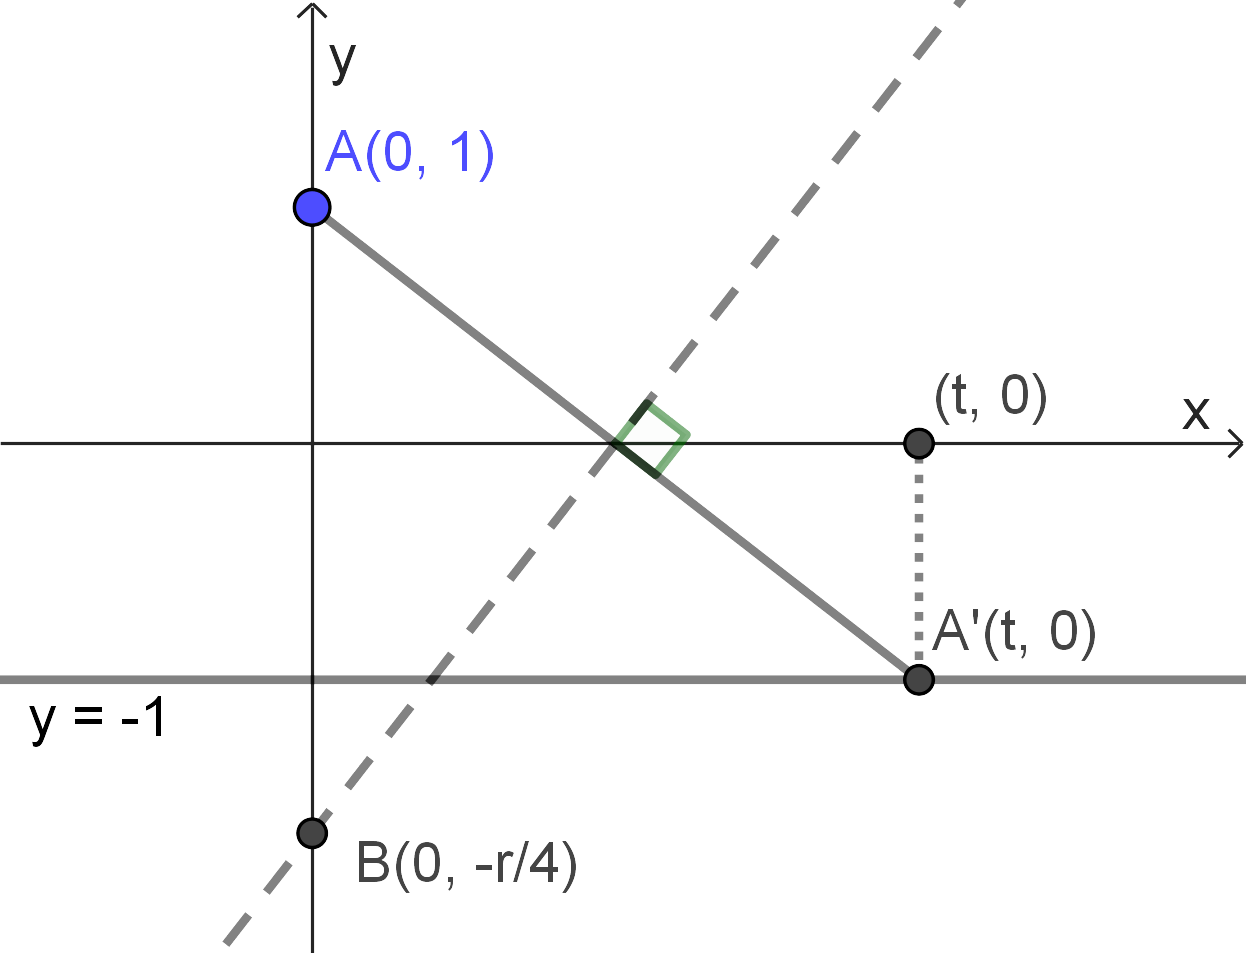
\includegraphics[width=0.5\textwidth]{images/kvadratni_koren.png}
    \caption[Konstrukcija korena]{Konstrukcija števila $\sqrt{r}$ za poljuben $r \in \Q^{+}$.}
    \label{fig:konstrukcija_korena}
\end{figure}

Pregib po konstrukciji poteka skozi točko $B$ in razpolovišče daljice $AA'$, torej je njegov koeficient $k_B = \frac{r}{2t}$ (izpeljavo prepuščamo bralcu). Ker je pregib simetrala daljice $AA'$, njena nosilka pa ima koeficient $k_A = - \frac{2}{t}$, dobimo
\begin{align*}
    k_B &= - \frac{1}{k_A},\\
    \frac{r}{2t} &= \frac{t}{2},\\
    r &= t^2 \text{ oz. } t = \sqrt{r}.
\end{align*}
Na koncu le še prepognemo pravokotnico na abscisno os skozi točko $A'$ in tako dobimo točko $(\sqrt{r}, 0)$. Torej smo konstruirali število $\sqrt{r}$ za poljuben $r \in $.

\subsection{Podvojitev kocke}
\label{podpogl:podvojitev_kocke}

Po legendi iz grške mitologije je bog Apolon po oraklju prebivalcem svojega rojstnega otoka Delosa sporočil, da mu morajo, če se želijo znebiti smrtonosne kuge, zgraditi nov oltar v obliki kocke, ki je enak prejšnjemu, le da mora biti dvakrat večji po prostornini. Torej je bilo potrebno konstruirati kocko s stranico, ki je za faktor $\sqrt[3][2]$ večja od stranice originalne kocke. Po drugi legendi pa naj bi Platon izjavil, da je ta problem, ki so ga prejeli na njegovi Akademiji v Atenah, poslan od bogov samih z namenom osramotiti Grke zaradi njihovega zanemarjanja in prezira do matematike (ker z evklidskim orodjem niso znali konstruirati poljubnih dolžin)~\cite[str.\ 29]{geometricconstructions}.

Ne vemo, ali so bili Grki prepričani, da se problema z neoznačenim ravnilom in šestilom ne da rešiti. Vsekako pa jim je manjkalo algebrsko znanje iz razdelka~\ref{podpogl:evkl_konstruktibilnost}.

\subsubsection*{Starogrška rešitev preko presečišča dveh parabol}

Mogoče Grkom ni uspelo priti do tega premisleka, vendar so problem vseeno uspeli rešiti, čeprav po drugi poti; uporabili so še eno močno matematično orodje -- stožnice. Videla v~\cite{videla1997} dokaže izrek, ki je identičen izreku~\ref{izr:orig_razp_polje} (ki govori, katera števila so origami števila), le da namesto origamija uporabi stožnice. V bistvu s tem dokaže, da so origami kosntrukcije ekvivalentne konstrukcijam s stožnicami!

V istem viru Videla tudi navaja konstrukcijo s parabolami, ki za dano dolžino $a$ podajo dolžino $c$, za katero velja $c^3 = a$. Njen avtor je Menehmo (prb.\ 350 pr.\ Kr.), tutor Aleksandra Velikega. Vzel je sledeči paraboli (slika~\ref{fig:videla}):
\begin{itemize}
    \item $\mathcal{P}_1: y = x^2$ z goriščem v točki $(0, \frac{1}{4})$ in premico vodnico $y = - \frac{1}{4}$ in
    \item $\mathcal{P}_1: x = \frac{y^2}{a}$ z goriščem v točki $(\frac{a}{4}, 0)$ in premico vodnico $x = - \frac{a}{4}$.
\end{itemize}
\begin{figure}[h]
    \centering
    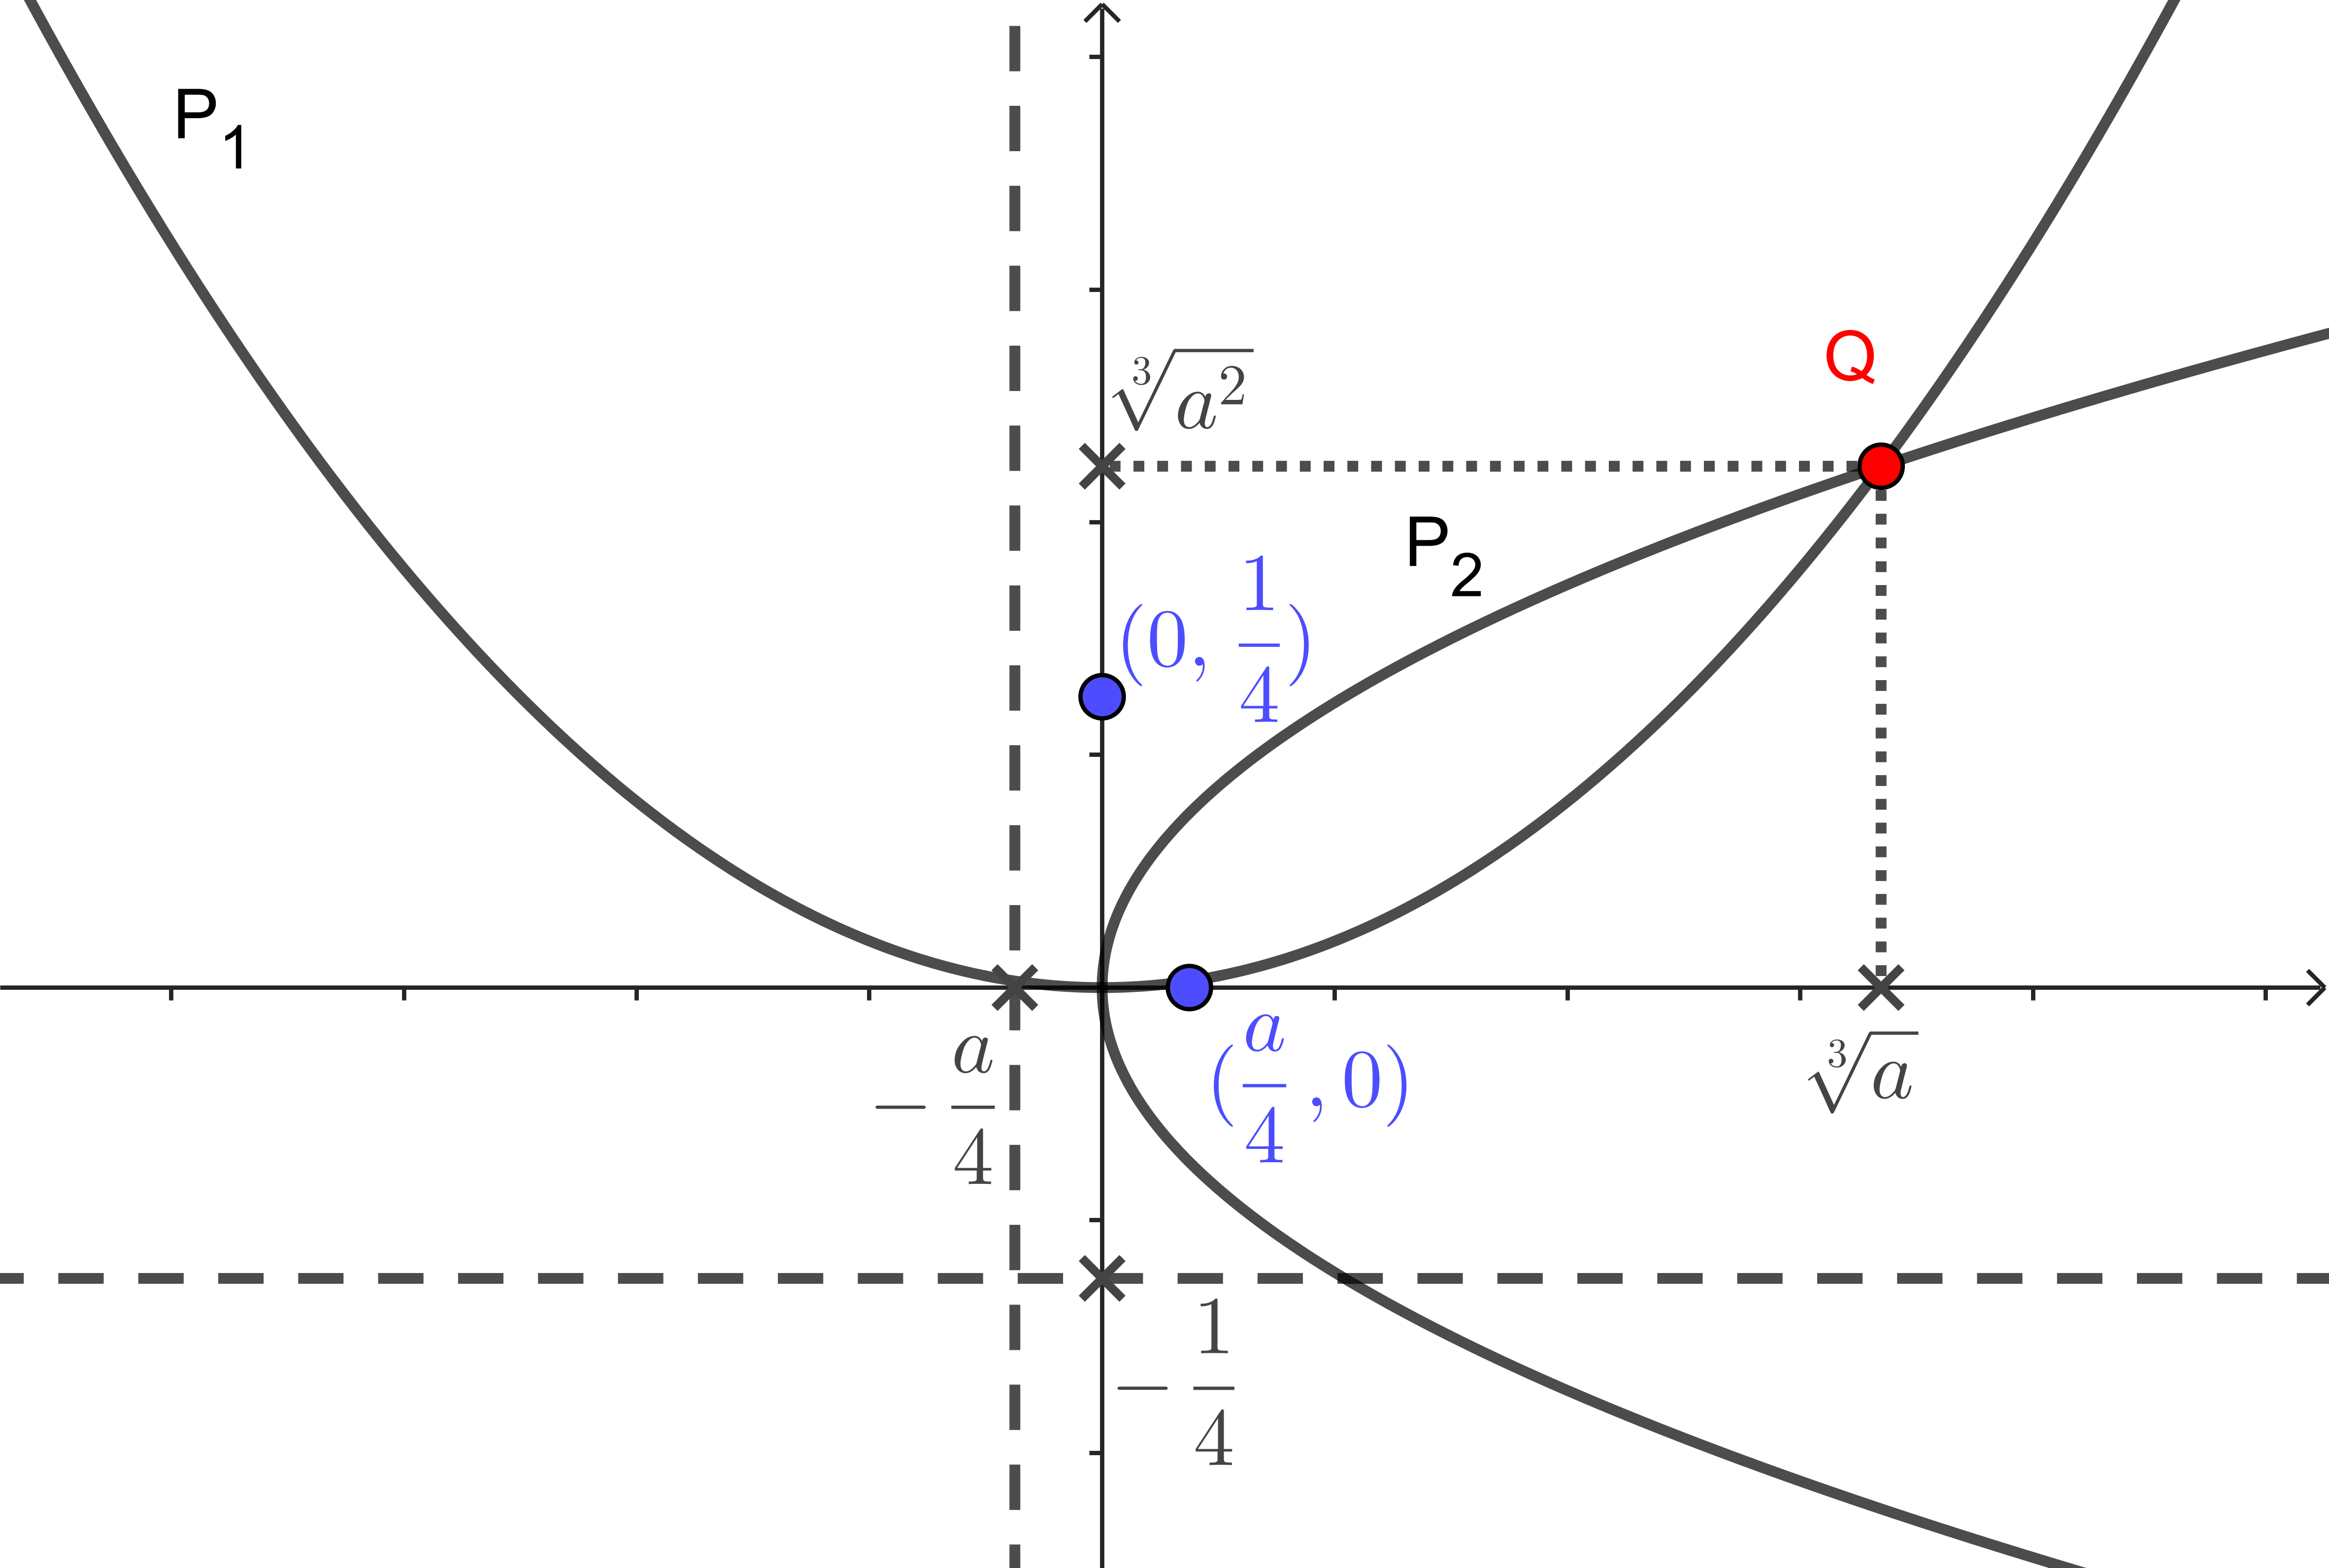
\includegraphics[width=0.7\textwidth]{images/starogr_problemi/cube_parabola.png}
    \caption[Menehmova konstrukcija kubičnega korena]{Menehmova konstrukcija števila $\sqrt[3]{2}$ preko parabol. Vzeto iz~\cite[str.\ 6]{videla1997}.}
    \label{fig:videla}
\end{figure}
Presečišči teh dveh parabol dobimo preko enakosti
$$y = x^2 = y^4/a^2,$$
kar nam da enačbo $y(a^2-y^3) = 0$ z rešitvama $y=0$ in $y = \sqrt[3]{a^2}$. Presečišči sta torej koordinatno izhodišče in točka $Q = (\sqrt[3]{a}, \sqrt[3]{a^2}) $. Njena abscisa je naša rešitev.
\opomba{Čeprav je konstrukcija enostavna in logična, je izvedljiva le v teoriji, saj z roko ne znamo natančno risati parabol.}

\subsubsection*{Martinova konstrukcija}

George E.\ Martin v~\cite[str.\ 156--157]{geometricconstructions} poda preprosto konstrukcijo števila $\sqrt[3]{k}$ za poljubno origami število $k$. Tudi on pri tem uporabi dve paraboli, vendar pri postopku potrebujemo le njuni gorišči in premici vodnici. Ne bomo iskali njunih presečišč, temveč bomo z Belochinim pregibom konstruirali njuno skupno tangento, ki nam bo podala željeni rezultat.

Naj bo $k \in $ poljuben. Vzemimo paraboli z goriščema v točkah $P = (-1, 0)$ in $Q = (0, -k)$ ter premici vodnici $p: x = 1$ in $q: y = k$. Paraboli imata skupno gorišče v koordinatnem izhodišču in sta pravokotni druga na drugo, torej imata eno samo skupno tangento. Prepognimo točko $P$ na premico $p$ in točko $Q$ na premico $q$. Pregib seka $y$-os v točki $R$ (slika~\ref{fig:martin}).
\begin{figure}[h]
    \centering
    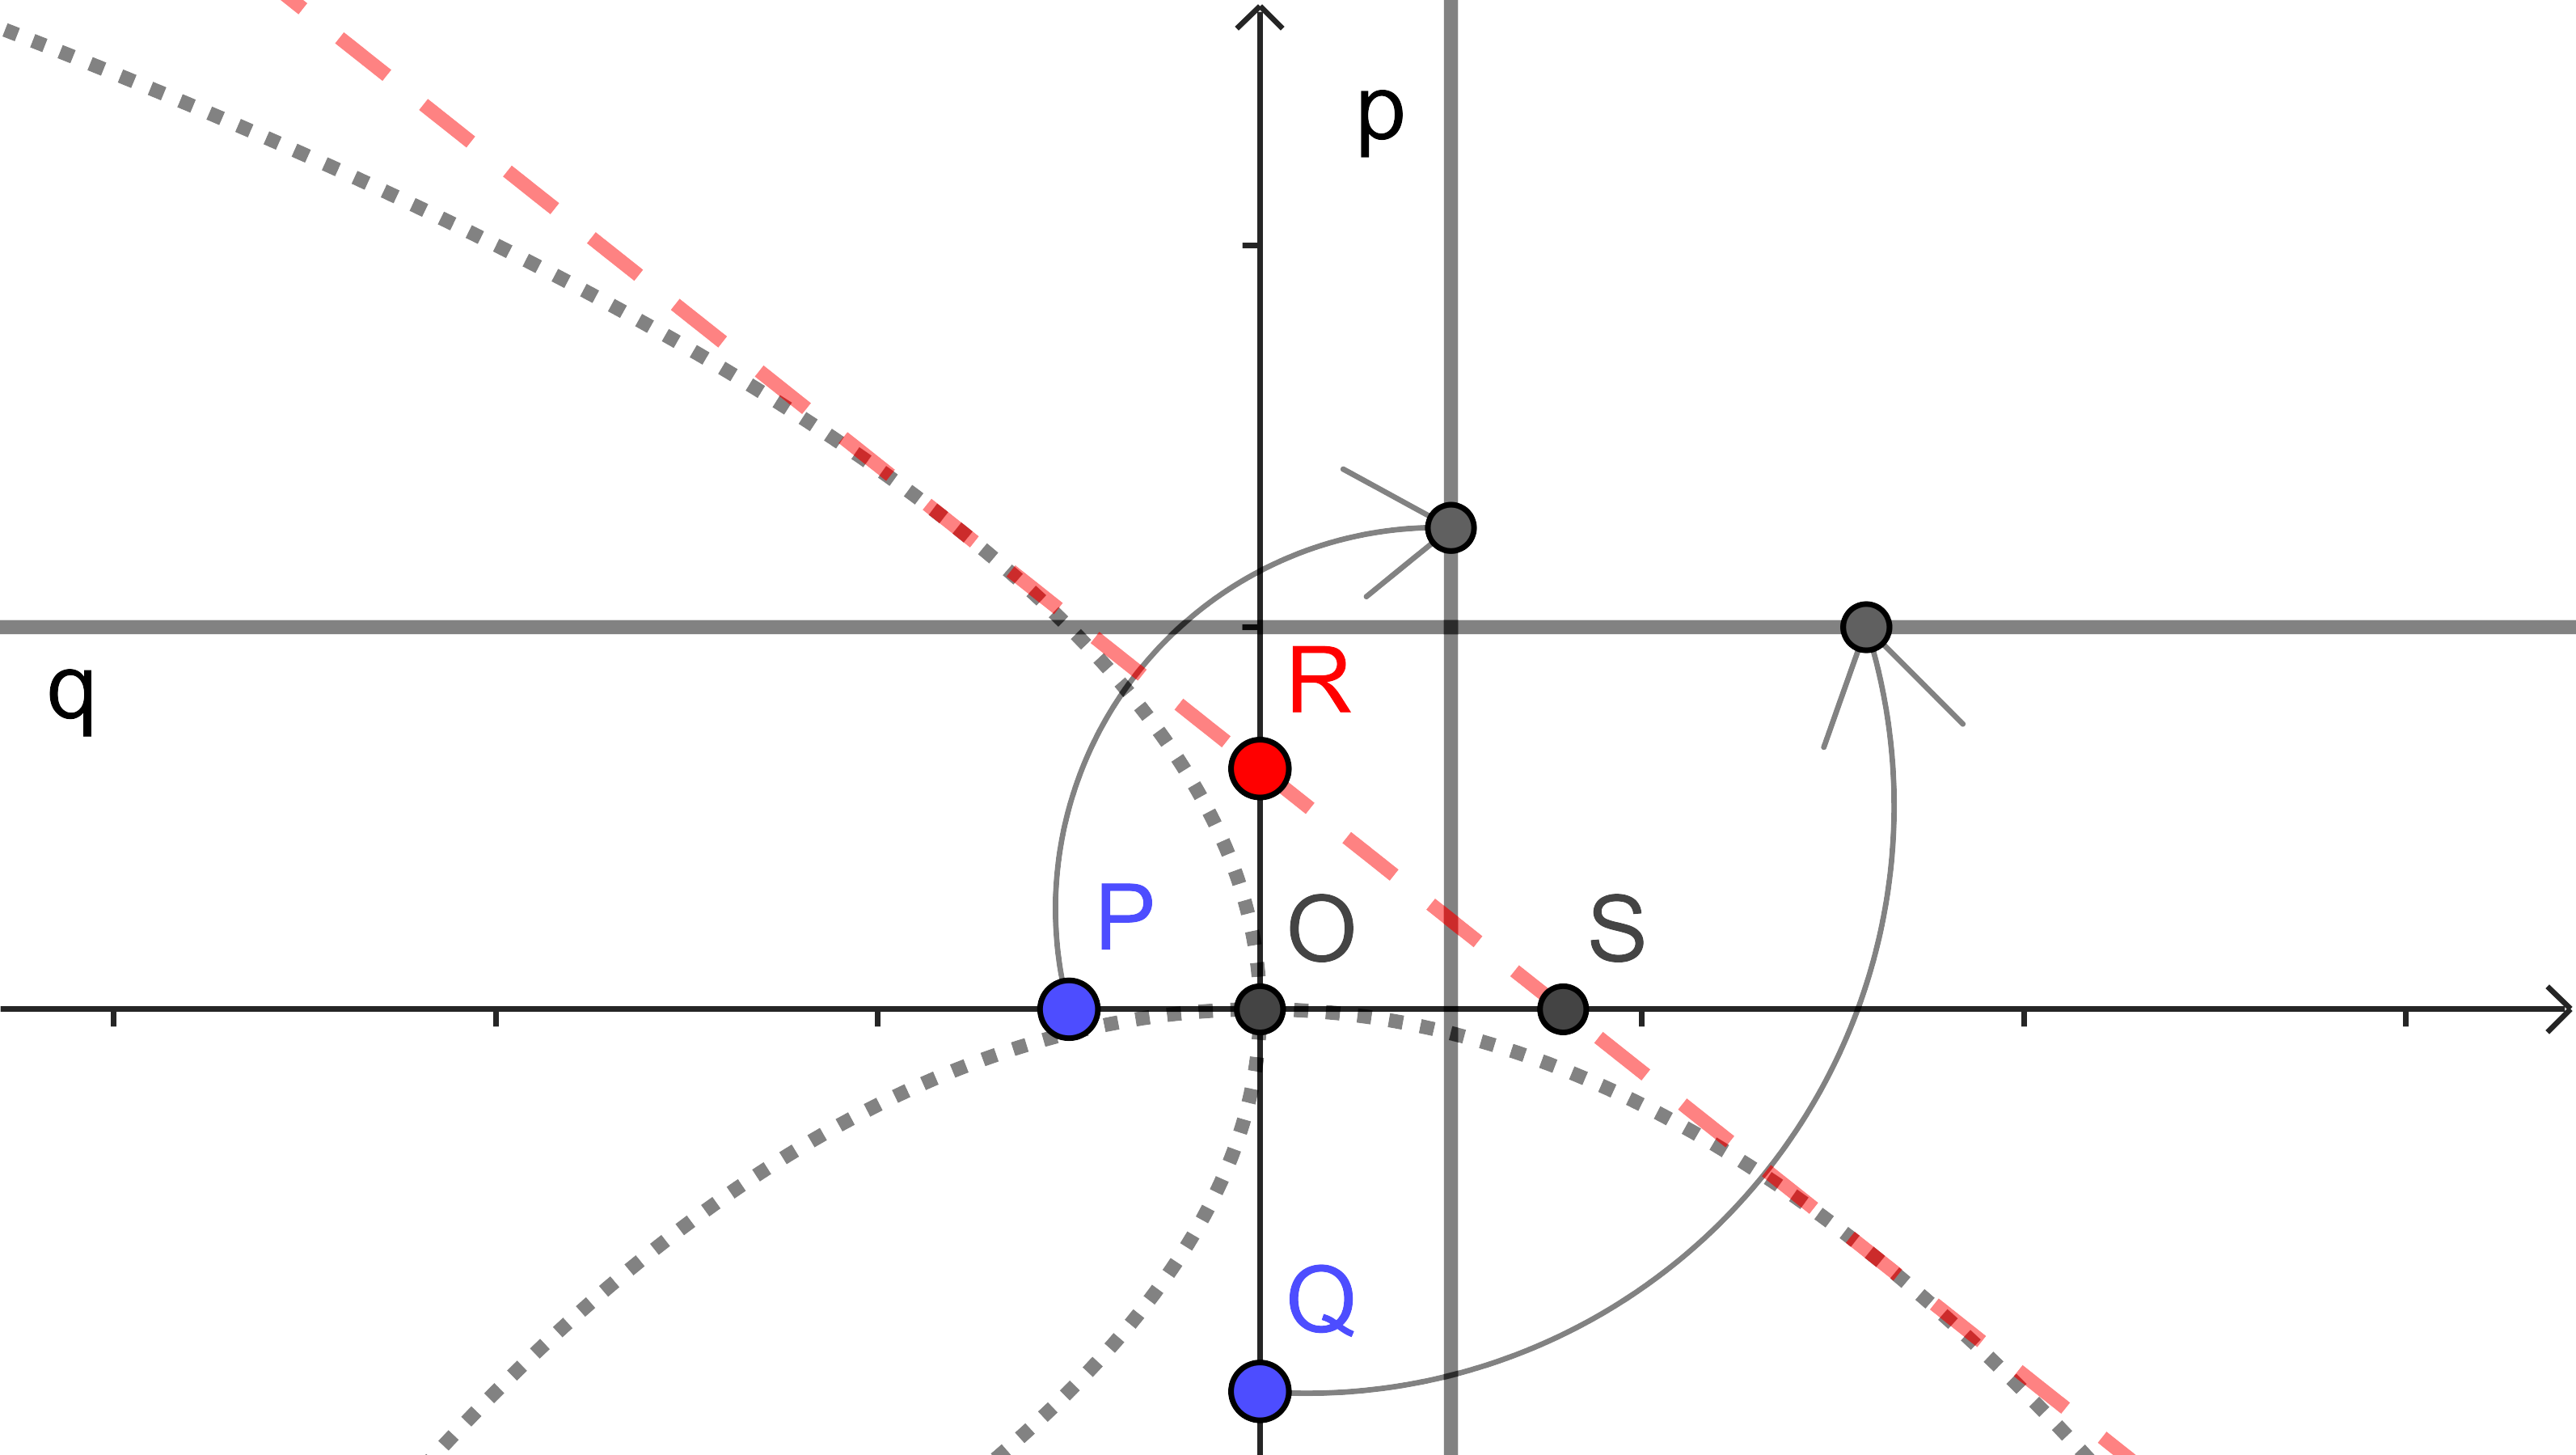
\includegraphics[width=0.6\textwidth]{images/starogr_problemi/cube_martin.png}
    \caption[Martinova konstrukcija kubičnega korena]{Martinova konstrukcija števila $\sqrt[3]{k}$.}
    \label{fig:martin}
\end{figure}
\begin{trditev}
    Točka $R$ iz zgornje konstrukcije ima koordinate $(0, \sqrt[3]{k})$.
\end{trditev}
\begin{dokaz}
    Označimo z $O$ koordinatno izhodišče in s $S$ presečišče pregiba z $x$-osjo. Točki $R$ in $S$ sta zaradi take izbire gorišč in premic vodnic ravno središči daljic z enim krajiščem v točkah $P$ in $Q$ ter drugim krajiščem v njunih slikah. Torej velja $PR \perp RS \perp SQ$. Zato so trikotniki $\triangle POR, \triangle ROS$ in $\triangle SOQ$ podobni. Iz tega ob upoštevanju $|OP| = 1$ in $|OQ| = k$ dobimo razmerje
    $$ \frac{|OR|}{|OP|} = \frac{|OS|}{|OR|} = \frac{|OQ|}{|OS|} \Longrightarrow |OR| = \frac{|OS|}{|OR|} = \frac{k}{|OS|}, $$
    iz česar sledi
    $$ |OR|^3 = |OR| \cdot \frac{|OS|}{|OR|} \cdot \frac{k}{|OS|} = k \Longrightarrow |OR| = \sqrt[3]{k}.$$
\end{dokaz}
\begin{opomba}
    V razdelku~\ref{podpogl:beloch_kvadrat_koren} bomo spoznali konstrukcijo števila $\sqrt[3]{2}$ preko Belochinega kvadrata, ki je v bistvu poseben primer Martinove konstrukcije.
\end{opomba}

\subsubsection*{Messerjeva konstrukcija}

Peter Messer v~\cite{messer1986} navaja avtorski postopek, ki sicer ne konstruira števila $\sqrt[3]{2}$ kot razdaljo, temveč kot razmerje: kvadraten list papirja po horizontali razdelimo na tri dele (to sedaj že znamo storiti) ter točki $p_1$ in $p_2$ s prepogibom položimo na premici $L_1$ in $L_2$, kot kaže slika~\ref{fig:messer} (levo).
\begin{figure}[h]
    \centering
    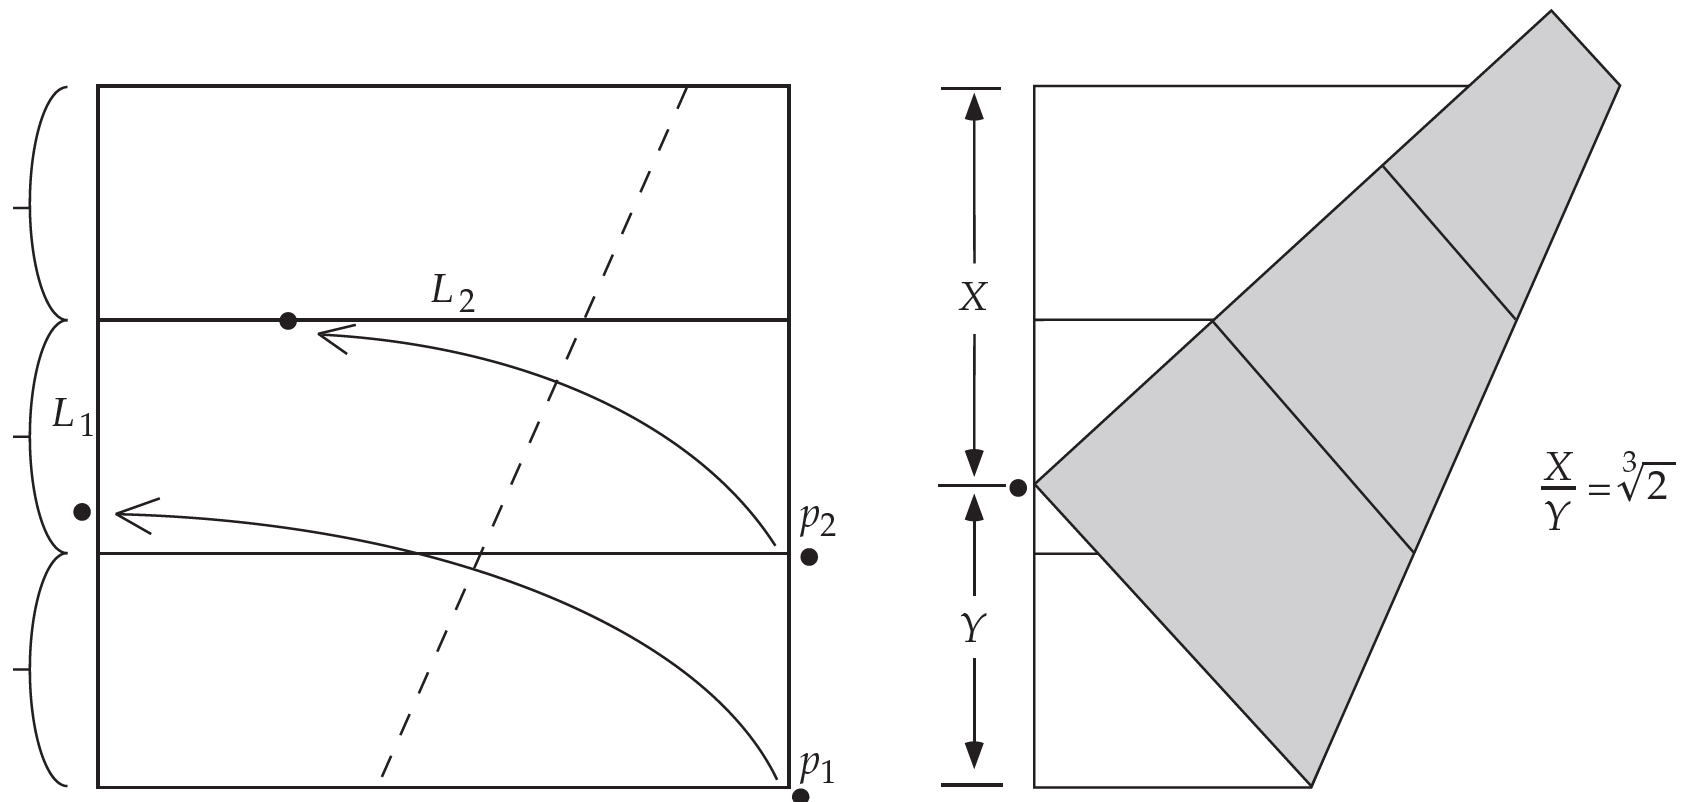
\includegraphics[width=0.68\textwidth]{images/starogr_problemi/messer1.png}
    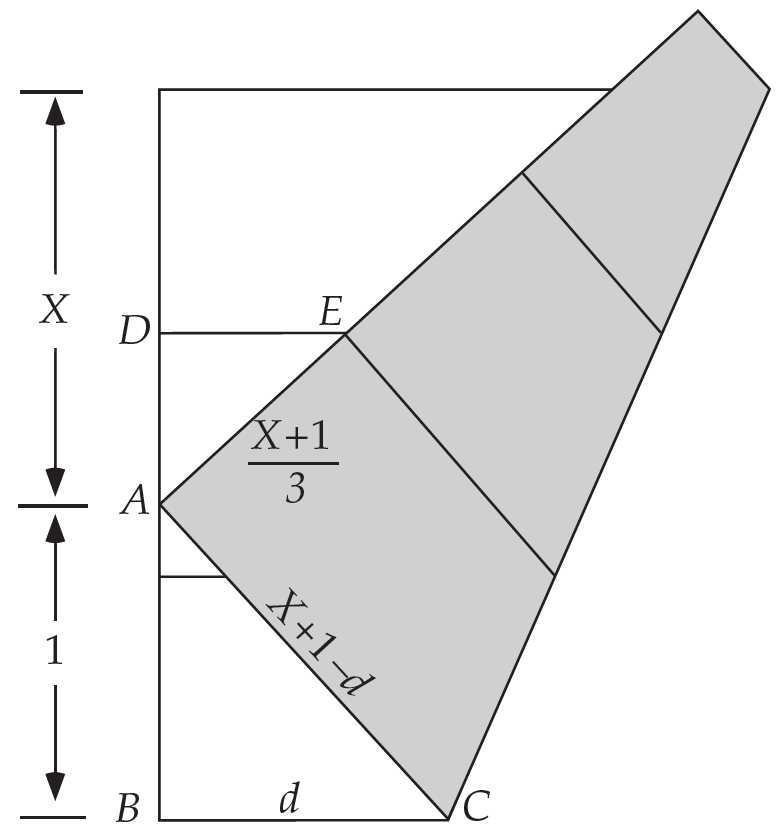
\includegraphics[width=0.3\textwidth]{images/starogr_problemi/messer2.png}
    \caption[Messerjeva konstrukcija]{Messerjeva konstrukcija razmerja $\sqrt[3]{2}$. Vzeto iz~\cite[str.\ 67--68]{hull2013}.}
    \label{fig:messer}
\end{figure}
\begin{trditev}
    Slika točke $p_1$ deli levo stranico kvadrata v razmerju $\sqrt[3]{2}$.
\end{trditev}
\begin{dokaz}
    Vpeljimo oznake $X, Y, A, B, C, D, E$ ter $d = |BC|$, kot kaže slika~\ref{fig:messer}. Dokazati moramo $X/Y = \sqrt[3]{2}$, za lažje računanje pa brez škode privzemimo $Y=1$. Stranica kvadrata je tako dolga $X+1$, zato je $|AC| = X+1-d$ in $|AE| = (X+1)/3$.

    Opazimo podobna pravokotnika $\triangle ABC$ in $\triangle ADE$. Iz trikotnika $\triangle ABC$ s pomočjo Pitagorovega izreka izrazimo $d = (X^2+2X)/(2X+2)$, preko leve stranice pa še $|AD| = X - (X+1)/3 = (2X-1)/3$. Iz podobnosti omenjenih trikotnikov izrazimo razmerje katete in hipotenuze z enačbo $|BC|/|AC| = |AD|/|AE|$. Ko vstavimo noter vse vrednosti, odvisne od $X$, dobimo enačbo
    $$ \frac{X^2 + 2X}{X^2 + 2X + 2} = \frac{2X - 1}{X + 1},$$
    ki se nam poenostavi prav v $X^3 = 2$. Torej je $X = \sqrt[3]{2}$.
\end{dokaz}
\opomba{Lahko bi rekli, da poleg razmerja v primeru $Y=1$ Messer konstruira razdaljo $\sqrt[3]{2}$, vendar je razdalja $Y$ odvisna od stranice kvadrata. V tem primeru bi morali vzeti kvadraten list papira s stranico $1 + \sqrt[3]{2}$, za kar bi pač potrebovali že konstrukcijo kubičnega korena števila $2$. Da bi pri splošnem kvadratnem listu papirja dobili to dolžino, moramo razdalji $X$ in $Y$ z origamijem še deliti, to pa že znamo.}

\subsection{Trisekcija kota}
\label{podpogl:trisekcija}

Kot $90^\circ$ znamo tretjiniti z neoznačenim ravnilom in šestilom, saj znamo konstruirati kot $30^\circ$. Vem pa že, da ne obstaja konstrukcija, s katero na tri skladne kote razdelimo \emph{poljuben} kot.

% SPODNJI DOKAZ JE PREPISAN IZ VIRA IN SAMO CITIRAN V prejšnjem odstavku

% Algebraični dokaz, da z evklidskim orodjem ne moremo tretjiniti poljubnega kota -- dokažimo za kot $60°$. (iz~\cite[str.\ 77--78]{jerman1998})

% Kot $60°$ znamo narisati. Če bi ga znali razdeliti na tri enake dele, bi potemtake znali narisati tudi kot $20°$, s tem pa (ker znamo risati pravokotnice) tudi $\cos 20°$ \textcolor{red}{slika z enotsko krožnico}. Pokažimo, da to ne gre.

% Izračunajmo minimalni polinom števila $\cos 20°$. Ker je
% $$ \frac{1}{2} = \cos 60° = \cos(3 \cdot 20°) = 4 \cos^3 20° - 3 \cos 20°, $$
% ima polinom $ p(x) = 8 x^3 - 6x - 1 $ ničlo $ \cos 20°$. Minimalni polinom števila $ \cos 20°$ deli polinom $p$. Če polinom $p$ razpade na produkt dveh polinomov s koeficienti v $\Q$, je eden od polinomov zagotovo linearen. To pa bi pomenilo, da ima polinom $p$ vsaj eno racionalno ničlo. Edini kandidatki za racionalne ničle polinoma $p$ so števila iz množice
% $$ \{\pm 1, \pm \frac{1}{2}, \pm \frac{1}{4}, \pm \frac{1}{8} \}. $$ Nobeno od teh števil ni ničla polinoma $p$, zato se $p$ ne da razcepiti na produkt dveh polinomov z racionalnimi koeficienti. Minimalni polinom števila $ \cos 20°$ je torej enaka
% $$ m(x) = \frac{1}{8} p(x) = x^3 - \frac{3}{4} x - \frac{1}{8}. $$
% Tako je razsežnost prostora $\Q(\cos 20°)$  nad obsegom $\Q$ enaka $3$ in števila $ \cos 20° $ se ne da narisati le z ravnilom in šestilom.

% Zato trisekcija kota v splošnem ni mogoča.

\subsubsection*{Starogrška rešitev preko presečišča krožnice in hiperbole}

Grki so tudi ta problem uspeli rešiti s stožnicami. Videla v~\cite[str.\ 6--7]{videla1997} opisuje Pappusovo konstrukcijo iz $3$.\ stoletja po Kr., ki je tu ne bomo dokazali. Gre za sledeč postopek: Na kraku $BA$ poljubnega kota $\angle ABC$ izberemo poljubno točko $F$ in zarišemo krožnico s središčem v točki $B$ in polmerom $BF$. Naj bo $BD$ simetrala kota $\angle ABC$. Naj bo presečišče krožnice in hiperbole z ekscentičnostjo $2$, ki ima gorišče v točki $F$ in premico vodnico $BD$, točka $E$ (slika~\ref{fig:trisection_gr}). Potem poltrak $BE$ tretjini kot $\angle ABC$.

\begin{figure}[h]
    \centering
    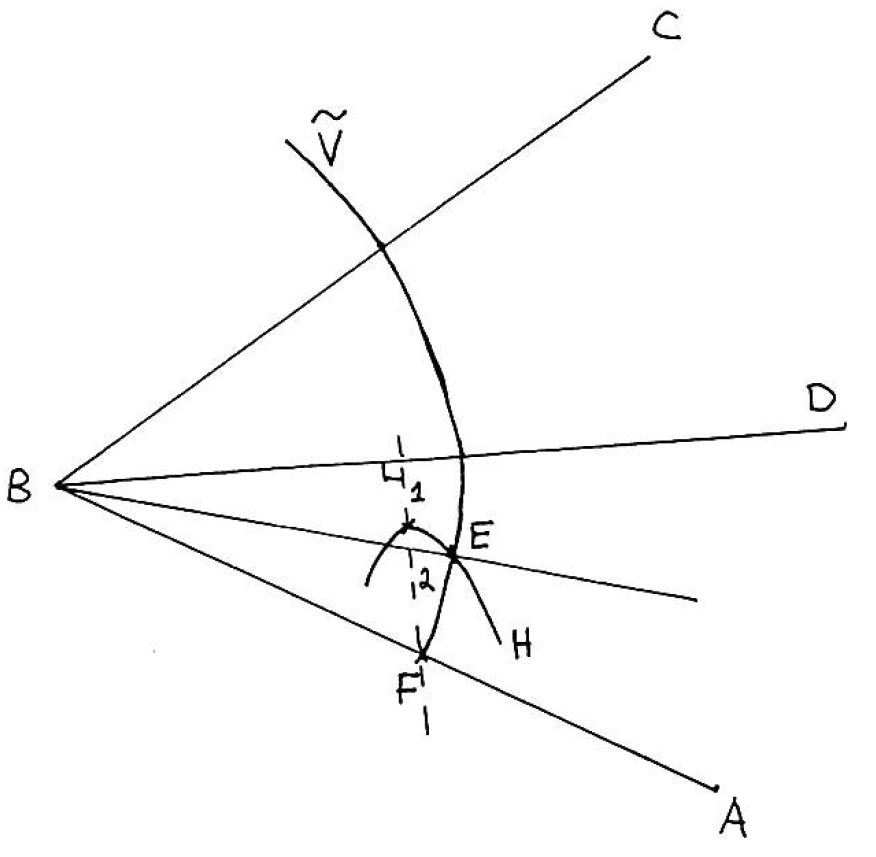
\includegraphics[width=0.5\textwidth]{images/starogr_problemi/trisection_grska.png}
    \caption[Pappusova trisekcija kota]{Pappusova trisekcija kota preko stožnic. Vzeto iz~\cite[str.\ 7]{videla1997}.}
    \label{fig:trisection_gr}
\end{figure}

\subsubsection*{Abejeva metoda}

Sledeča metoda ima ime po japonskemu matematiku Hisashiju Abeju, ki jo je odkril v $80$-ih letih prejšnjega stoletja. Postopek vključuje Belochin pregib, torej se ga ne da izvesti z evklidskim orodjem, edina pomankljivost metode pa je, da deluje le za ostre kote. Postopek je sledeč:

\begin{enumerate}
    \item Na kvadratnem listu papirja konstruiramo poljuben kot $\theta$, ki ima vrh v spodnjem desnem vogalu in en krak na spodnji stranici. Nato konstruiramo še dva horizontalna in ekvidistančna pregiba na dnu papirja (slika~\ref{fig:abe_1} levo).
    \item Točko $p_1$ prepognemo na spodnji horizontalen pregib, označen $L_1$, točko $p_2$ pa na poševen krak kota, označen z $L_2$ (slika~\ref{fig:abe_1} na sredi).
    \item Preden pregib razgrnemo, podaljšamo pregib $L_1$ do konca in nov pregib označimo z $L_3$ (slika~\ref{fig:abe_1} desno).
    \item Papir razgrnemo in tokrat v spodnji levi kot podaljšamo pregib $L_3$.
\end{enumerate}
\begin{figure}[h]
    \centering
    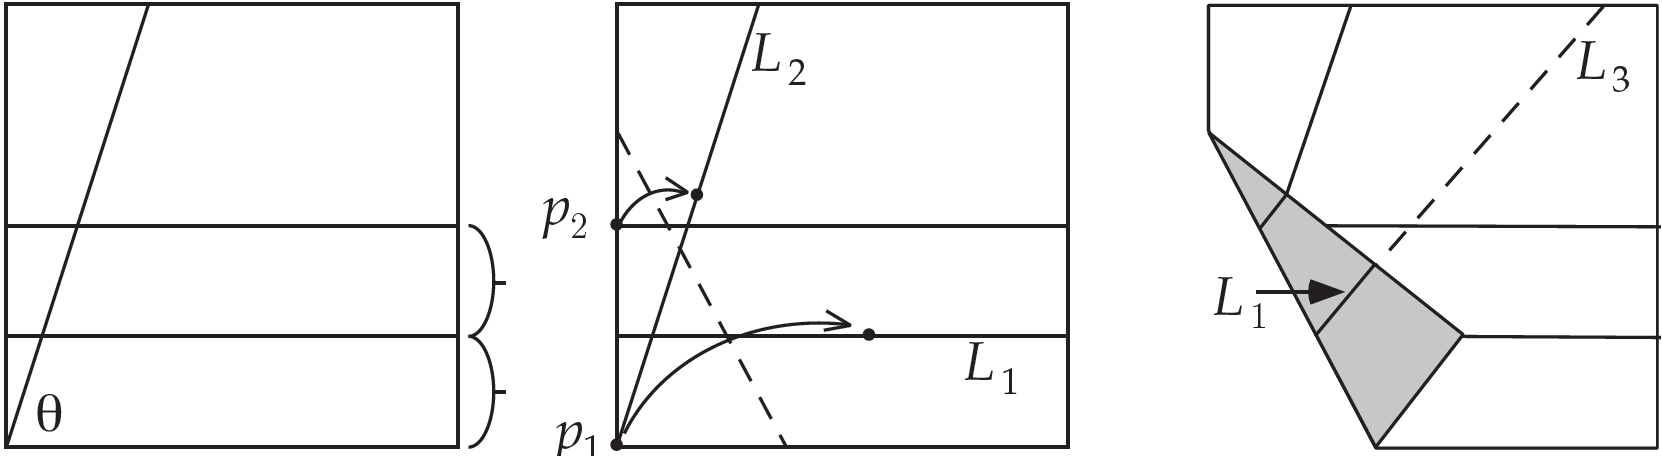
\includegraphics[width=0.95\textwidth]{images/starogr_problemi/abe_nastavek1.png}
    \caption[Abejeva metoda ($1$.\ del)]{Trisekcija kota po Abejevi metodi. Vzeto iz~\cite[str.\ 64]{hull2013}.}
    \label{fig:abe_1}
\end{figure}

\opomba{V $3$.\ koraku opravimo pregib še preden smo razgrnili prvega. To je za nas načeloma prepovedana poteza, vendar bi se dalo $L_3$ konstruirati tudi po klasični poti z enkratnimi prepogibi -- označili bi sliko točke, ki leži hkrati na $L_1$ in levi stranici kvadrata, ter točko v pregibu iz $2$.\ koraka, ki leži na $L_1$ in skozinju naredili pregib $L_3$ -- zato zaradi lažje izvedbe brez škode dopustimo tak postopek.}

\begin{trditev}
    Pregib $L_3$ poteka skozi točko $p_1$. Kot s krakoma $L_2$ in $L_3$ ter vrhom v točki $p_1$ je velik $\theta/3$.
\end{trditev}
\begin{posledica}
    Ko spodnji rob kvadrata prepognemo na pregib $L_3$, razdelimo kot $\theta$ na tri skladne kote.
\end{posledica}

\begin{dokaz}
    Posledica logično sledi, zato dokazujemo le trditev. Označimo z $x$ točko, ki leži na presečišču pregiba $L_1$ in pregiba iz $2$.\ koraka Abejeve metode. Z $A, B$, in $C$ označimo še slike točk z leve stranice kvadrata, kot kaže slika~\ref{fig:abe_2}.
    \begin{figure}[h]
        \centering
        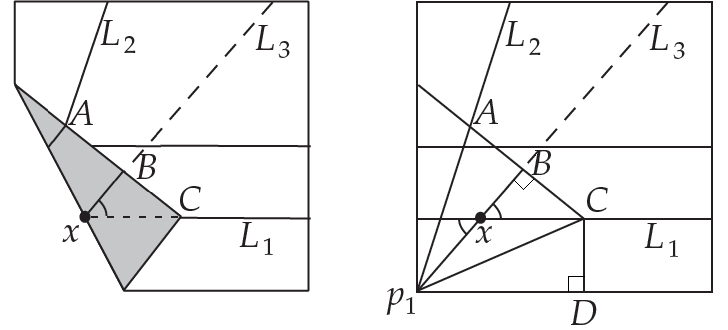
\includegraphics[width=0.7\textwidth]{images/starogr_problemi/abe_trisekcija.png}
        \caption[Abejeva metoda ($2$.\ del)]{Dokazovanje Abejeve metode. Vzeto in predelano iz~\cite[str.\ 65]{hull2013}.}
        \label{fig:abe_2}
    \end{figure}
    Ker je točka $C$ slika točke $p_1$ in $x$ leži na $L_1$, daljica $xC$ leži na $L_1$. Po konstrukciji daljica $xB$ leži na $L_3$, zato sta kota ob $x$, ko papir razgrnemo, skladna. Zaradi sovršnosti kotov daljica $p_1x$ leži na $L_3$, s čimer je prvi del trditve dokazan.
    
    Na razgrnjenem papirju zarišemo (ali prepognemo) še nekaj daljic (slika~\ref{fig:abe_2} desno). Ker velja $|AB| = |BC| = |CD|$ in imata pravokotna trikotnika $\triangle p_1AB$ in $\triangle p_1BC$ skupno še drugo kateto, trikotnika $\triangle p_1BC$ in $\triangle p_1CD$ pa skupno hipotenuzo, so vsi trije trikotniki skladni z enakim kotom v točki $p_1$, torej nam pregiba skozi daljici $p_1B$ (kar je ravno $L_3$) in $p_1C$ kot $\theta$ razdelijo na tri skladne kote.
\end{dokaz}

Ker ta postopek deluje le za ostre kote, si poglejmo naslednjo metodo, ki jo lahko uporabljamo tako za ostre kot tudi tope kote.

\subsubsection*{Justinova metoda}

Francoski matematik Jacques Justin za svojo metodo trisekcije ne zahteva kvadratnega lista papirja, ampak je dovolj kakršenkoli list. Lang v~\cite[str.\ 34]{lang2013} takole navaja njegovo kosntrukcijo:

Na sredo narišemo poljuben kot $\angle ABC$ (oster ali top) in njuna kraka podaljšamo skozi vrh $B$. Skozi vrh konstruiramo poltrak, pravokoten na krat $BA$. Točko $C$ prezrcalimo čez vrh v točko $D$ ter nato obe točki prepognemo na nosilko kraka $BA$ in ravno konstruirano pravokotnico, kot kaže slika~\ref{fig:justin} (levo). Nazadnje na Belochin pregib konstruiramo še pravokotnico skozi točko $B$.
\begin{figure}[h]
    \centering
    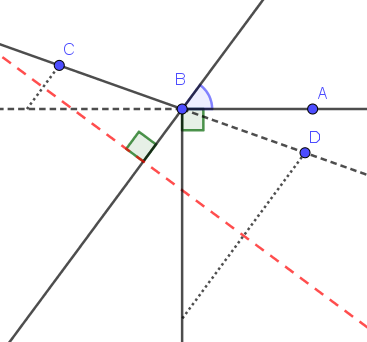
\includegraphics[width=0.45\textwidth]{images/starogr_problemi/justin_trisection.png}
    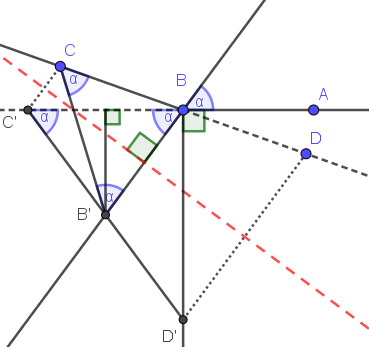
\includegraphics[width=0.45\textwidth]{images/starogr_problemi/justin_trisection_dokaz.png}
    \caption[Justinova trisekcija kota]{Justinova trisekcija kota (levo) in njen geometrijski dokaz (desno).}
    \label{fig:justin}
\end{figure}

\begin{trditev}
    Kot, ki v točki $B$ oklepata zadnja pravokotnica iz zgornje konstrukcije in krak $BA$, je tretjina kota $\angle ABC$.
\end{trditev}
\begin{dokaz}
    Označimo z $\alpha$ kot iz trditve. Naj bosta točki $C'$ in $D'$ sliki točk $C$ in $D$, točka $B'$ pa presečišče daljice $C'D'$ s pravokotnico iz trditve. Po konstrukciji Belochinega pregiba je daljica $C'D'$ slika daljice $CD$, torej je točka $B'$ slika točke $B$. Točka $B'$ je tako središče daljice $C'D'$ in zato je vzporednica k poltraku $BD'$ skozi točko $B'$ simetrala daljice $C'B$. Trikotnik $\triangle C'B'B$ je tako enakokrak in velja $\angle C'BB' = \angle B'C'B = \alpha$.
    
    Ker sta trikotnika $\triangle C'B'B$ in $\triangle CBB'$ zaradi simetričnosti glede Belochin pregib skladna, velja tudi $\angle B'CB = \angle CB'B = \alpha$. Iz vsote notranjih kotov trikotnike $\triangle CB'B$ sledi $\angle C'BC = 180^\circ - 3\alpha$, torej je $\angle ABC = 180^\circ - \angle C'BC = 3\alpha$. 
\end{dokaz}

\subsubsection*{Martinovi konstrukciji za trisekcijo ostrega kota}

George E.\ Martin v~\cite[poglavje 10]{geometricconstructions} navaja še dve metodi za trisekcijo ostrega kota.

Pri prvi vzamemo oster kot $\angle PQR$ in s točko $M$ označimo središče daljice $PQ$. Skozi $M$ konstruiramo pravokotnico $p$ na $QR$, nato pa še pravokotnico na $p$. Opravimo tisti Belochin pregib (od treh možnih), ki seka daljico $PM$ in točko $Q$ položi na premico $q$ (v točko $Q'$), točko $P$ pa na premico $p$ (v točko $P'$). S $T$ označimo presečišče daljice $QQ'$ s premico $p$ in s $S$ presečišče pregiba s premico $q$ (slika~\ref{fig:trisection_10.4}).

\begin{figure}[h]
    \centering
    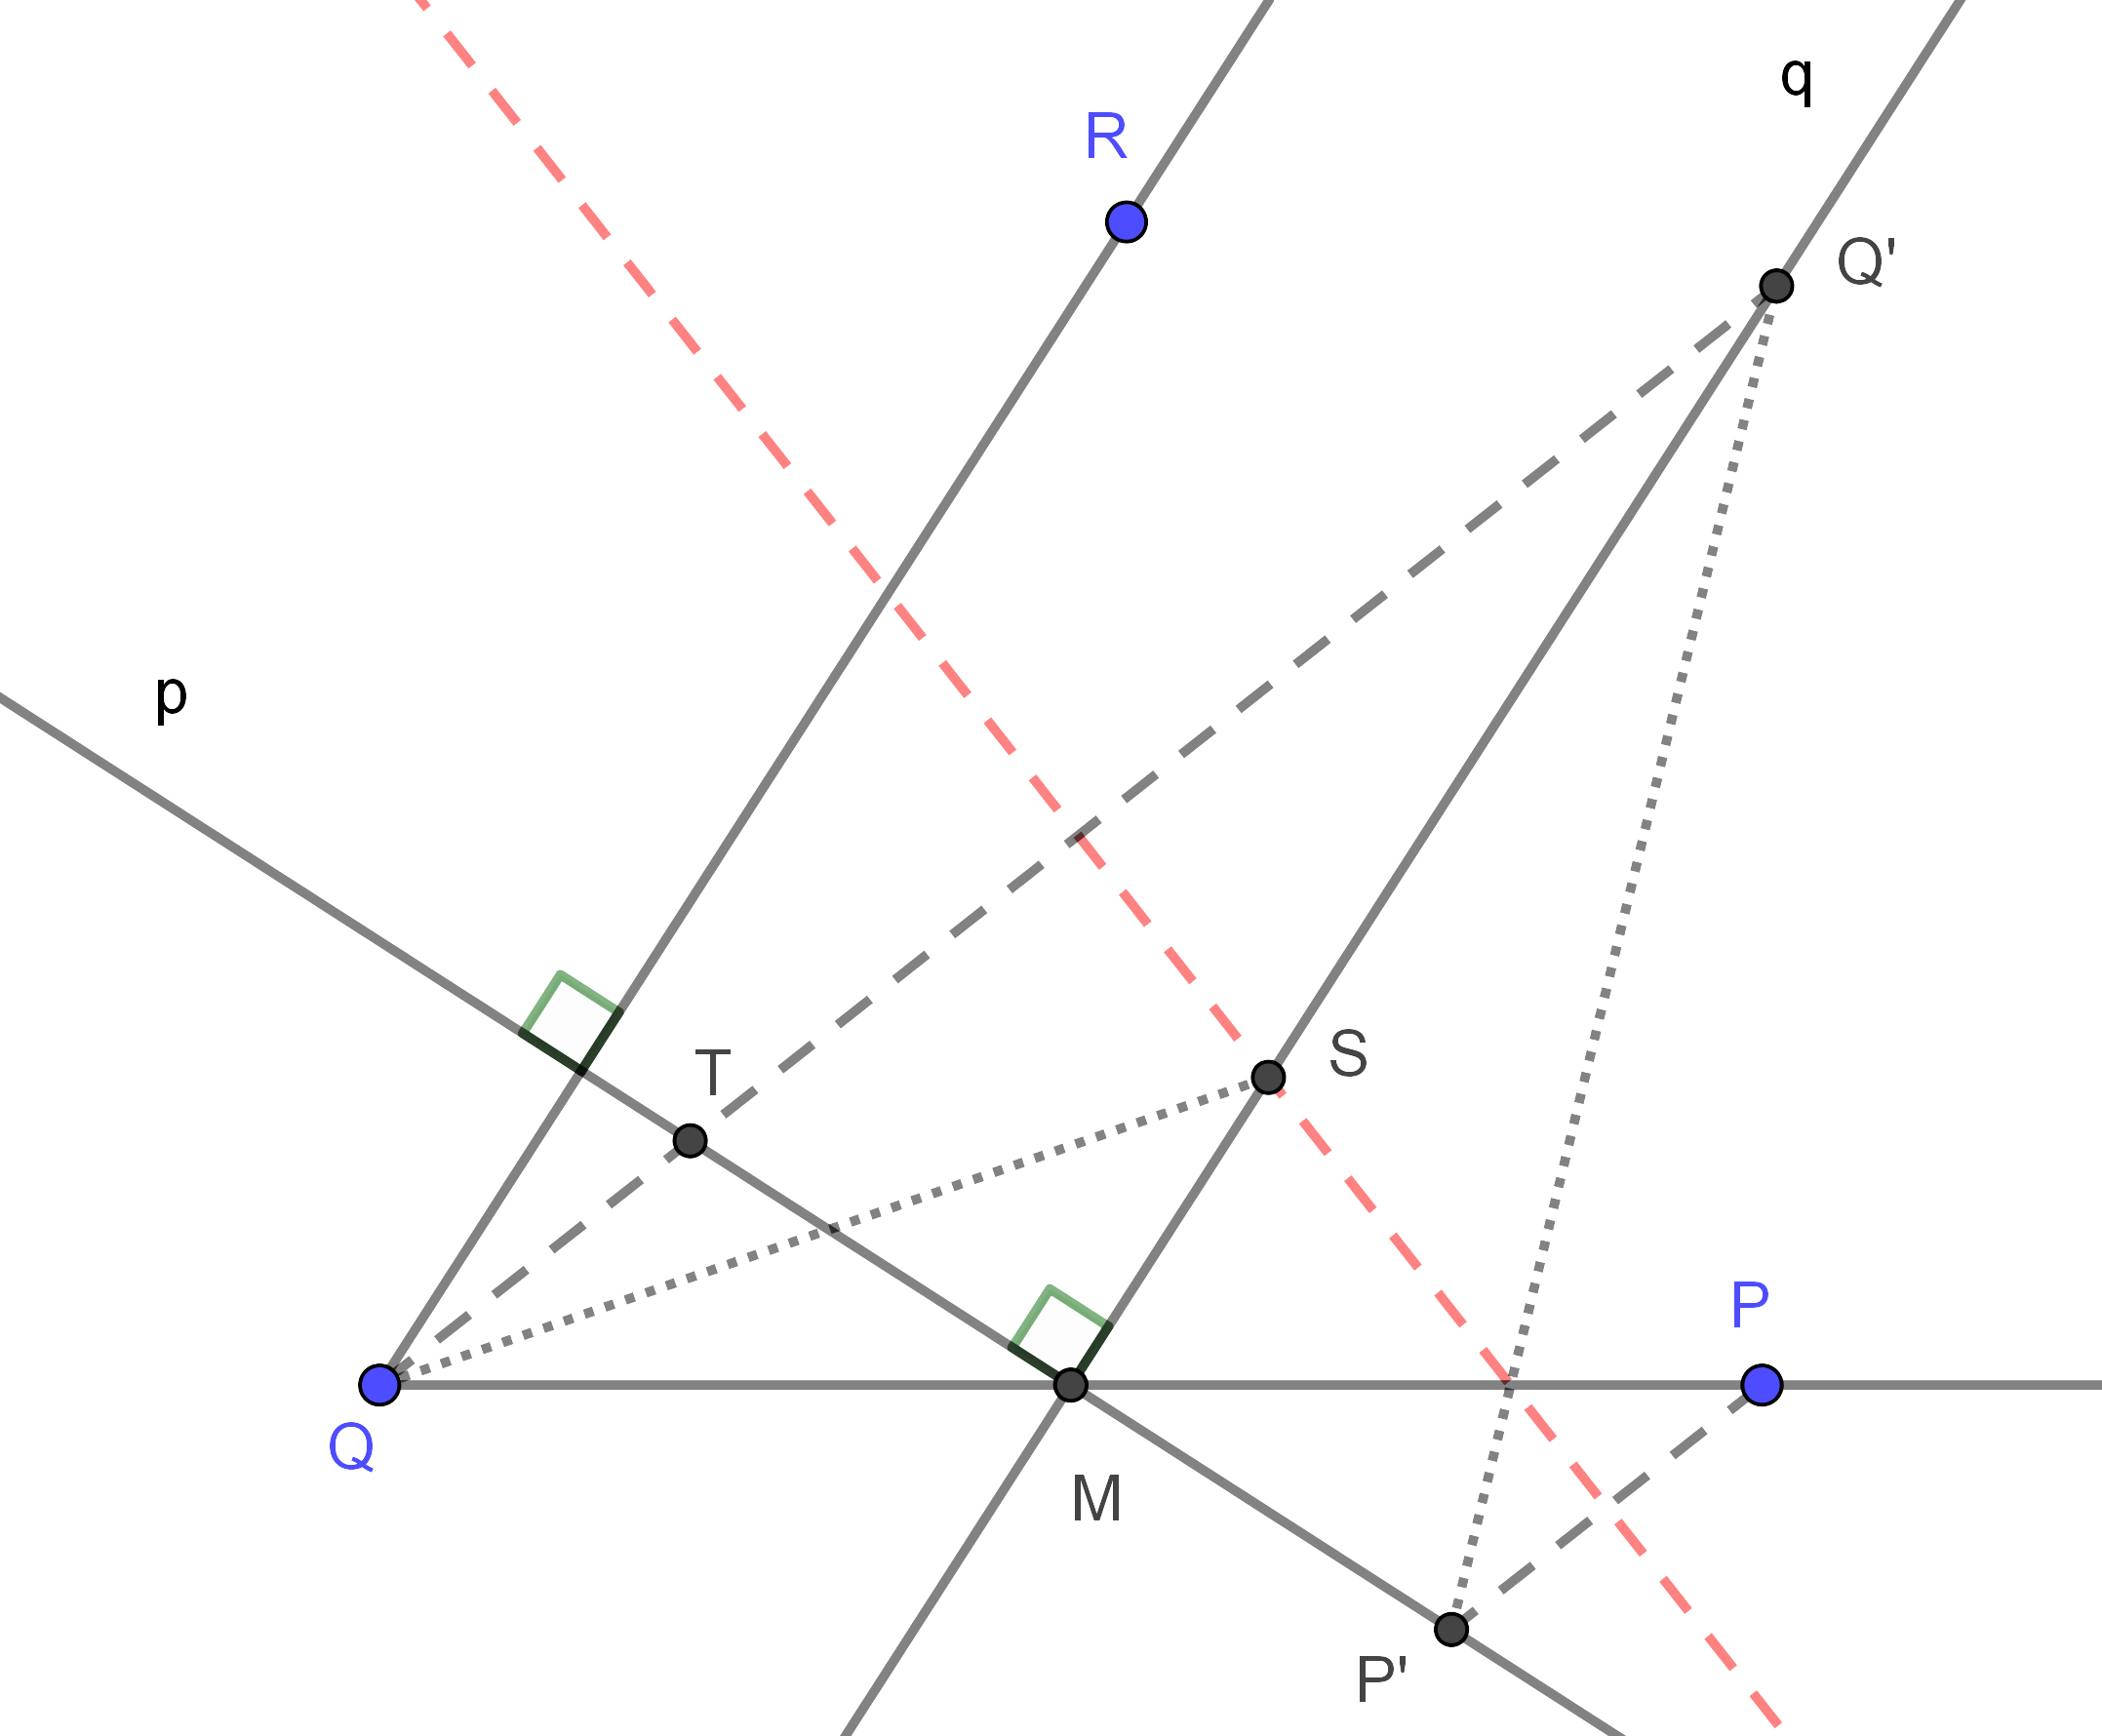
\includegraphics[width=0.5\textwidth]{images/starogr_problemi/trisection_10.4.png}
    \caption[Martinova trisekcija ostrega kota (metoda $1$)]{Martinov postopek za trisekcijo kota iz~\cite[str.\ 154]{geometricconstructions}.}
    \label{fig:trisection_10.4}
\end{figure}

\begin{trditev}
    Daljici $QT$ in $QS$ tretjinita kot $\angle PQR$.
\end{trditev}
\begin{dokaz}
    Ker velja $|QM| = |MP|$, $\angle PMP' = \angle TMQ$ in $QT \parallel PP'$, sta trikotnika $\triangle QMT$ in $\triangle PMP'$ skladna in je $|TM| = |MP'|$. Potem sta skladna tudi pravokotna trikotnika $\triangle TMQ'$ in $\triangle P'MQ'$, zato je $\angle MQ'P' = \angle TQ'M = \angle RQQ'$ (zaradi izmeničnih kotov ob vzporednicah $QR$ in $q$) $= \angle Q'QS$ (ker je trikotnik $\triangle QSQ'$ enakokrak).
    
    Bralec se lahko hitro prepriča, da daljica $Q'P'$ seka pregib ravno v njegovem presečišču z daljico $MP$ (vsi koti ob tem presečišču so zaradi konstrukcija pregiba in sovršnosti skladni). Zato velja še $\angle PQQ' = \angle P'Q'Q$, iz česar sledi
    $$ \angle MQS = \angle SQT = \angle TQR.$$
\end{dokaz}

Druga metoda je prvi zelo podobna. Zopet vzamemo oster kot $\angle PQR$ in s točko $M$ označimo središče daljice $PQ$. Naj bo $l$ pravokotnica na $QR$ skozi točko $Q$, točka $N$ nožišče pravokotnice na premico $l$ skozi točko $P$, s $q$ označimo pa še pravokotnico na premico $l$ skozi točko $M$. Opravimo tisti Belochin pregib, ki točko $Q$ položi na premico $q$ (v točko $Q'$) in točko $N$ na poltrak $QR$. Naj bo točka $S$ presečišče pregiba s premico $q$ (slika~\ref{fig:trisection_10.14}).

\begin{figure}[h]
    \centering
    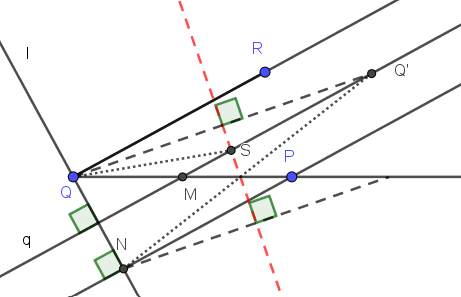
\includegraphics[width=0.6\textwidth]{images/starogr_problemi/trisection_10.14.png}
    \caption[Martinova trisekcija ostrega kota (metoda $2$)]{Martinov postopek za trisekcijo kota iz~\cite[str.\ 158--159]{geometricconstructions}.}
    \label{fig:trisection_10.14}
\end{figure}

\begin{trditev}
    Daljici $QQ'$ in $QS$ tretjinita kot $\angle PQR$.
\end{trditev}
\begin{dokaz}
    Zopet premislimo, da se pregib, poltrak $QP$ in daljica $NQ'$ sekajo v isti točki. Zato je $\angle QQ'N = \angle PQQ'$. Zaradi vzporednosti kraka $QR$ in premice $q$ sta skladna tudi izmenična kota $\angle RQQ'$ in $\angle QQ'S$, z njima pa je zaradi enakokrakosti trikotnika $\triangle QSQ'$ skladen tudi kot $\angle SQQ'$.

    Ker velja $|QM| = |MP|$ in $q \parallel NP$, je premica $q$ simetrala daljice $QN$, torej tudi simetrala kota $\angle QQ'N$. Iz tega sledi
    $$ \angle MQS = \angle SQQ' = \angle Q'QR.$$
\end{dokaz}